\documentclass[10pt,twocolumn,letterpaper]{article}

\usepackage[margin=0.75in,columnsep=0.3125in]{geometry}
\usepackage{times}
\usepackage[T1]{fontenc}
\usepackage{amsmath,amssymb}
\usepackage{graphicx}
\usepackage{booktabs}
\usepackage{algorithm}
\usepackage{algpseudocode}
\usepackage[font=small,labelfont=bf]{caption}
\usepackage[colorlinks=true,linkcolor=blue!60!black,citecolor=green!40!black,urlcolor=blue!60!black]{hyperref}

\newcommand{\R}{\mathbb{R}}
\newcommand{\Hhat}{\hat{H}}
\newcommand{\Ohat}{\hat{O}}
\newcommand{\Dhat}{\hat{\Delta}}

\title{\textbf{SA-VM: Scene Augmentation with Cross-Sample View Mixing\\for Multi-View Pedestrian Detection and Tracking}}
\author{Rizwan Khan}
\date{}

\begin{document}
\maketitle

\begin{abstract}
Early-fusion multi-view detectors lift image features from several calibrated cameras into a shared bird's-eye-view
(BEV) representation and detect and track pedestrians on the ground plane. On the standard WILDTRACK benchmark they
are trained on only 360 annotated frames of a single scene, which makes them prone to overfitting to the crowd layouts
and to the exact camera geometry seen during training. We propose SA-VM, an early-fusion network trained with two transformations of the
reference frame in which each camera is lifted. Scene augmentation
mirrors the reference frame of each training sample, jointly for all views and the labels. Cross-sample view mixing
then lifts a fixed subset of the cameras of each sample with the reference frame of the other sample in the batch,
so that in two thirds of the training batches three of the seven views carry evidence that disagrees with the labels
while four agree. The network is thereby trained to rely on agreement across views. We describe an evaluation protocol with seed-paired statistical comparison against an identically
retrained baseline, an ablation of each component, a camera-dropout control, and a robustness study under
calibration noise and camera failure.
\end{abstract}

%-----------------------------------------------------------------------------------------------------------------
\section{Method}
\label{sec:method}

Figure~\ref{fig:overview} gives an overview. SA-VM is an early-fusion detection and tracking network with
bilinear-sampling feature lifting~\cite{teepe2024lifting,harley2023simplebev}, trained with two transformations of
the reference frame in which each camera is lifted. Sec.~\ref{sec:problem} states the problem and
Sec.~\ref{sec:network} describes the network. Scene augmentation (Sec.~\ref{sec:sa}) transforms the reference frame
per sample, and cross-sample view mixing (Sec.~\ref{sec:vm}) assigns reference frames per camera.
Sec.~\ref{sec:loss} gives the training objective and Sec.~\ref{sec:inference} inference and tracking.

\begin{figure*}[t]
  \centering
  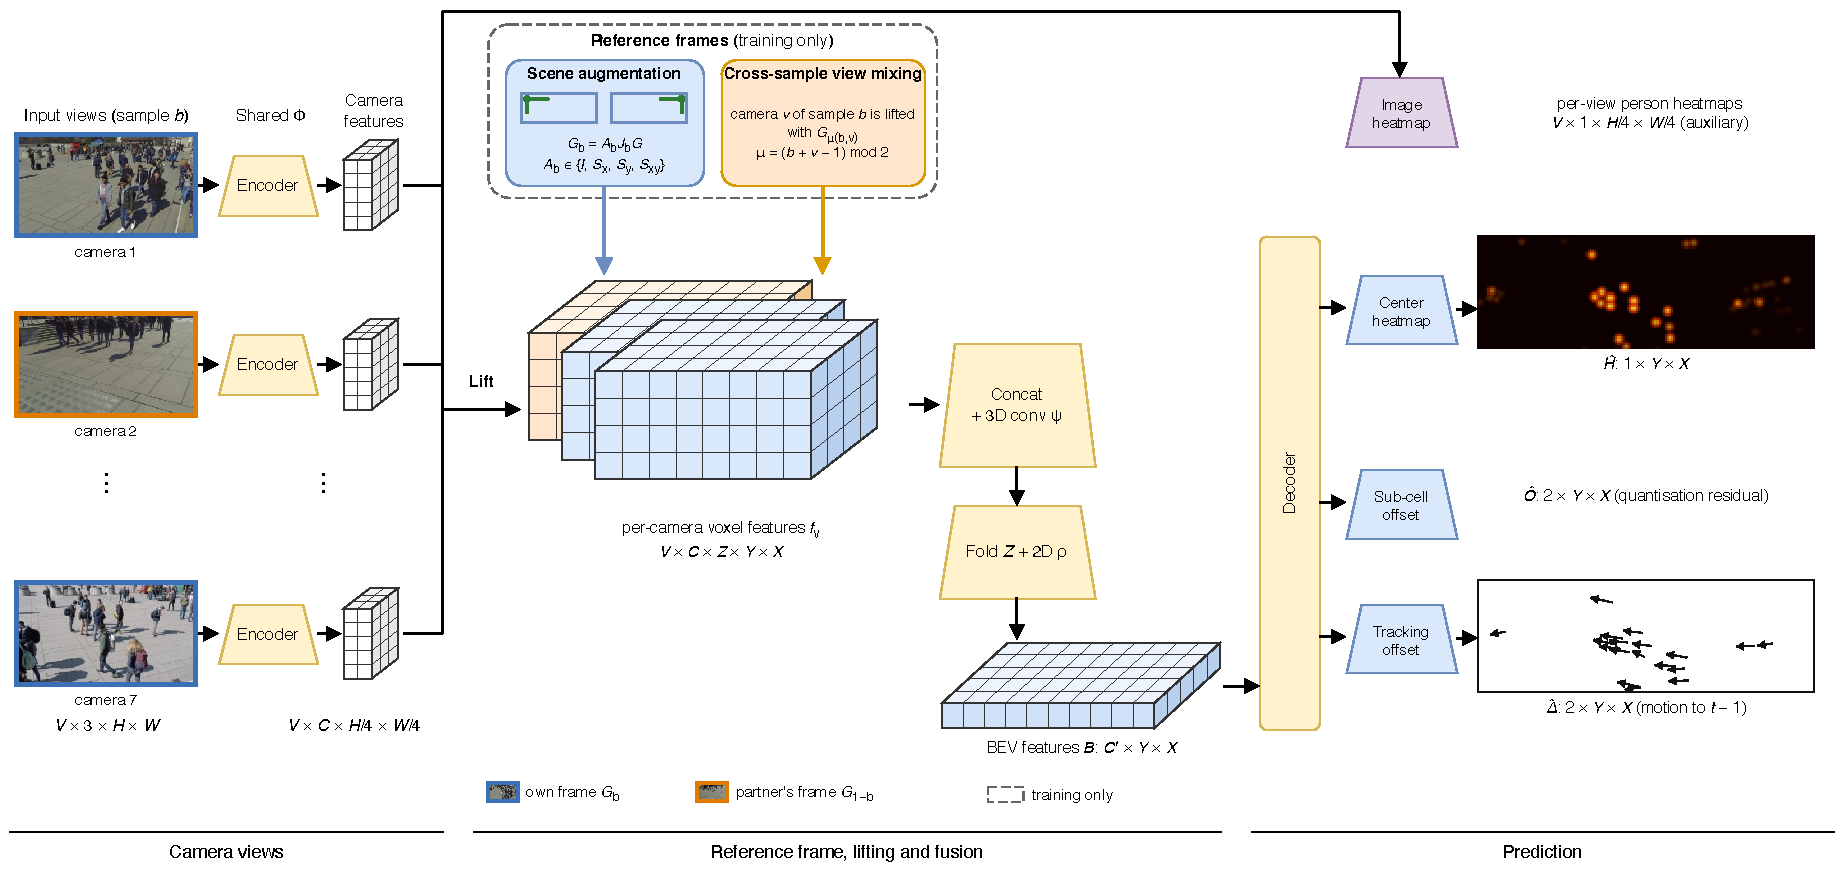
\includegraphics[width=\textwidth]{figures/fig1_overview.pdf}
  \caption{\textbf{Overview of SA-VM.} The $V$ synchronised views are encoded by a shared encoder $\Phi$. Camera
  features are lifted into a voxel grid by bilinear sampling, fused by concatenation and a 3D convolution $\psi$,
  and compressed into a BEV feature map $B$. The decoder predicts a centre heatmap $\Hhat$, sub-cell offsets
  $\Ohat$ and tracking offsets $\Dhat$; an auxiliary head predicts per-view heatmaps. During training (dashed box),
  scene augmentation transforms the reference frame $G_b$ of each sample, and cross-sample view mixing lifts the
  cameras marked in orange with the reference frame of the other sample in the batch. At inference every camera is
  lifted with the untransformed reference frame. Input pictures are WILDTRACK training frames; the prediction
  panels show the detections of a trained SA-VM model on test frame 360 and its tracking offsets, magnified
  $12\times$ for visibility.}
  \label{fig:overview}
\end{figure*}

\subsection{Problem formulation}
\label{sec:problem}

A scene is observed by $V$ static, synchronised cameras with intrinsics $K_v$ and extrinsics
$T_v = [R_v \,|\, t_v]$, $v \in \{1,\dots,V\}$. A fixed similarity transform $G$ maps world coordinates to the
reference frame of the ground plane, which is discretised into $X \times Y$ cells, with $Z$ height bins. Given the
images $I_{1:V}$ at time $t$, the model predicts the ground-plane position of every pedestrian and its displacement
to the position at time $t-1$. A tracker links these detections into trajectories with persistent identities.

\subsection{Detection and tracking network}
\label{sec:network}

\paragraph{Image encoder.} Each image is resized to $720 \times 1280$ and encoded by a
ResNet-18~\cite{he2016resnet}, pre-trained on ImageNet and shared by all cameras, with frozen batch-normalisation
statistics. The stem and the first three residual stages produce features at 1/4, 1/8 and 1/16 of the input
resolution. The 1/16 features are upsampled twice by bilinear interpolation, concatenated first with the 1/8 and then
with the 1/4 features, and mixed by $1 \times 1$ convolutions. A final $1 \times 1$ convolution gives the camera
features $\Phi(I_v) \in \R^{C \times H/4 \times W/4}$ with $C = 128$ ($180 \times 320$).

\paragraph{Feature lifting.} The ground plane is covered by a grid of $X \times Y \times Z = 360 \times 120 \times 4$
voxels of $10 \times 10 \times 50$\,cm, spanning $36 \times 12 \times 2$\,m. For the centre $\mathbf{x}$ of a voxel in
the reference frame, camera $v$ contributes the feature
\begin{equation}
  f_v(\mathbf{x}) = \Phi(I_v)\big\langle \pi\big(\tilde{K}_v\, T_v\, G^{-1}\, \mathbf{x}\big) \big\rangle,
  \label{eq:lift}
\end{equation}
where $\pi$ is the perspective division, $\tilde{K}_v$ is the intrinsic matrix scaled to the feature resolution and
$\langle\cdot\rangle$ denotes bilinear interpolation~\cite{harley2023simplebev}. Voxels that project outside the
image receive a zero feature. Every voxel along a camera ray therefore receives the feature of the pixel the ray
passes through, and a pedestrian is localised where the rays of several cameras agree.

\paragraph{Multi-view fusion.} The $V$ lifted feature volumes are concatenated along the channel axis in a fixed
camera order ($V C = 896$ channels). The fusion $\psi$ is a $3 \times 3 \times 3$ convolution to $C$ channels,
followed by instance normalisation, a ReLU and a $1 \times 1 \times 1$ convolution. The $Z = 4$ height bins are then
folded into the channels, and the compressor $\rho$, a $3 \times 3$ convolution with instance normalisation and a ReLU
followed by a $1 \times 1$ convolution, produces the BEV feature map
\begin{equation}
  B = \rho\Big(\mathrm{fold}_Z\big(\psi([f_1; \dots; f_V])\big)\Big) \in \R^{C' \times Y \times X},
  \label{eq:fuse}
\end{equation}
with $C' = 256$. Because the concatenation order is fixed, $\psi$ can weight each camera individually.

\paragraph{Temporal block.} Two convolutions combine $B$ with the BEV map of the previous frame. In all our
configurations the temporal memory is disabled, so the block receives $B$ in both inputs.

\paragraph{BEV decoder.} An encoder--decoder with ResNet-18 stages processes the BEV map. A $7 \times 7$ stride-2
convolution and three residual stages downsample it by a factor of 8, and three bilinear upsampling stages with skip
connections restore the full $120 \times 360$ resolution.

\paragraph{Heads.} Each head is a $3 \times 3$ convolution with 128 channels, instance normalisation and a ReLU,
followed by a $1 \times 1$ convolution. The centre head predicts the heatmap $\Hhat \in [0,1]^{Y \times X}$; its bias
is initialised to $-2.19$, a prior probability of 0.1. The offset head predicts four channels: the sub-cell offset
$\Ohat \in \R^{2 \times Y \times X}$, which recovers the quantisation residual of each cell, and the tracking offset
$\Dhat \in \R^{2 \times Y \times X}$ from each pedestrian's current position to its position at $t-1$. An image head
of the same form on the camera features predicts a per-view person heatmap $\Hhat^{\mathrm{img}}_v$ at 1/4
resolution, which guides the features before they are lifted~\cite{teepe2024lifting}.

\subsection{Scene augmentation}
\label{sec:sa}

With only 360 training frames from a single scene, the network sees a small number of crowd layouts. Scene
augmentation~\cite{engilberge2023mvaug} creates new layouts by transforming the reference frame rather than the
images. For training sample $b$ we use
\begin{equation}
  G_b = M_b\, J_b\, G, \qquad M_b = C\, S_b\, C^{-1},
  \label{eq:sa}
\end{equation}
where $C$ translates the origin to the centre of the grid, $S_b \in \{I, S_x, S_y, S_{xy}\}$ with
$S_x = \mathrm{diag}(-1, 1)$, $S_y = \mathrm{diag}(1, -1)$ and $S_{xy} = \mathrm{diag}(-1,-1)$ acting on the
ground-plane coordinates, and $J_b$ is a small random translation drawn uniformly from $[-0.25, 0.25]^2$ grid cells.
$S_b = I$ with probability $0.5$; otherwise one of the three mirrors is drawn uniformly
(Fig.~\ref{fig:savm}a). Mirrors about the grid centre map the grid onto itself, so no annotated pedestrian leaves the
area, unlike general affine scene transformations~\cite{engilberge2023mvaug}. The same transform is applied to the
ground-plane labels of frames $t$ and $t-1$,
\begin{equation}
  y_b = M_b J_b\, y, \qquad y_b^{t-1} = M_b J_b\, y^{t-1},
  \label{eq:sa_labels}
\end{equation}
so the tracking targets remain consistent with the detection targets. The images and the image-plane labels are not
modified. Since Eq.~\eqref{eq:lift} is evaluated with $G_b$ in place of $G$ for every camera, the lifted evidence of
all views moves together with the labels, and the transformed sample is geometrically consistent.

\begin{figure*}[t]
  \centering
  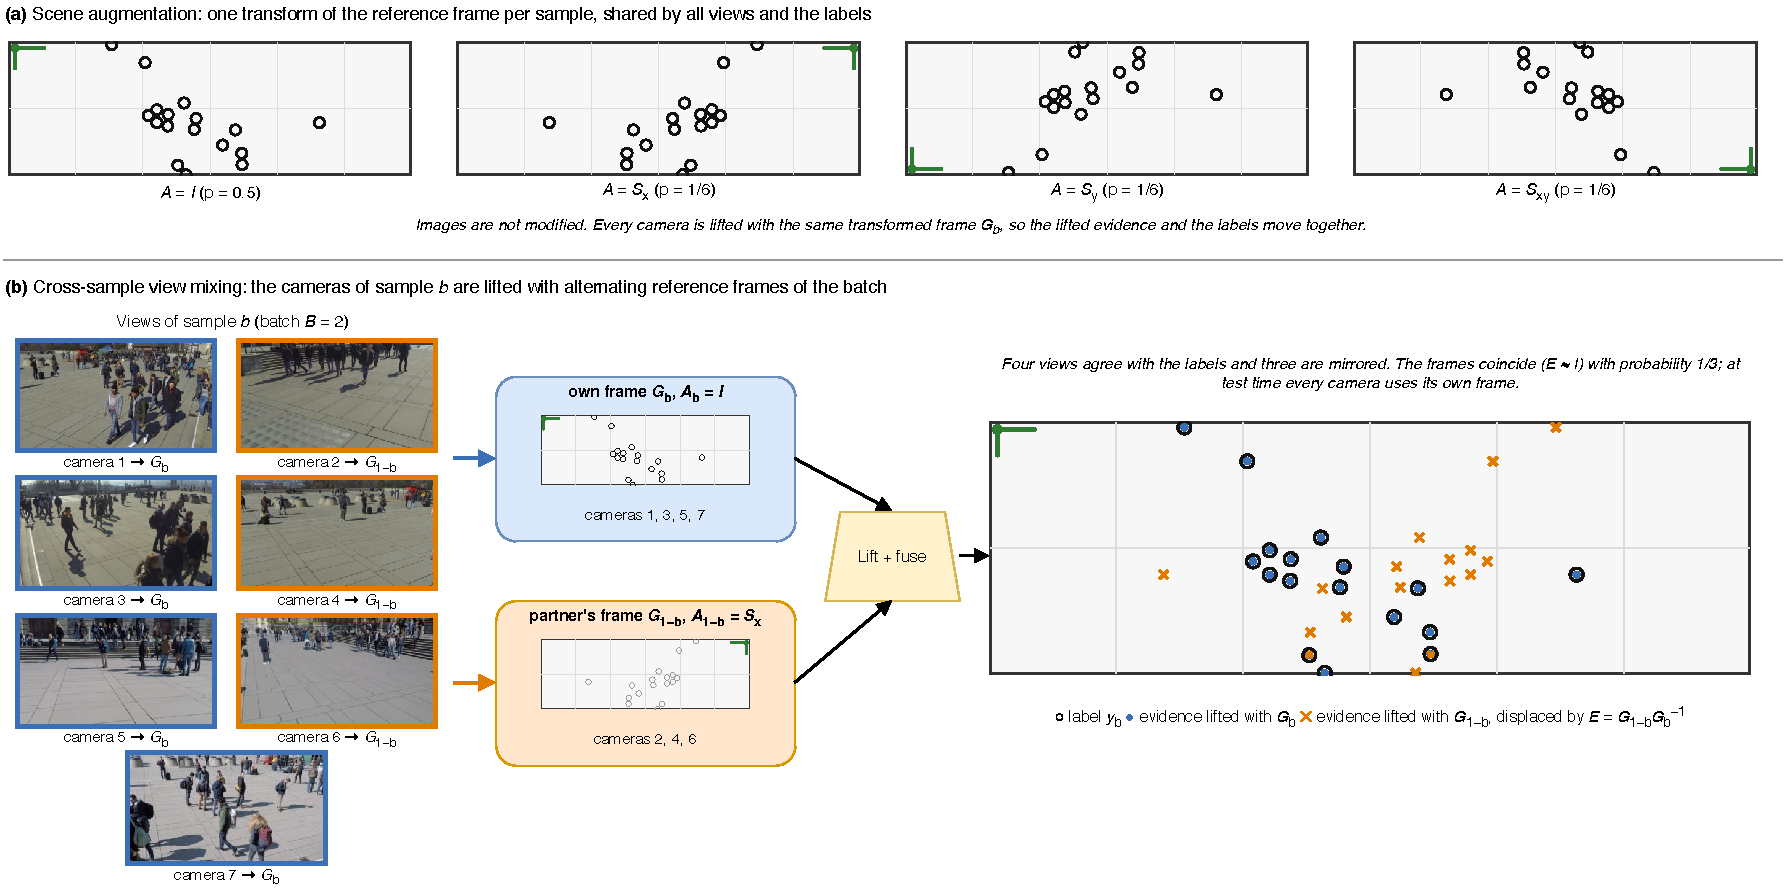
\includegraphics[width=\textwidth]{figures/fig2_sa_vm.pdf}
  \caption{\textbf{Scene augmentation and cross-sample view mixing.} (a) The four reference frames of
  Eq.~\eqref{eq:sa}, shown with the ground-truth positions of one WILDTRACK frame; the green marker is the origin
  and the axes of the untransformed frame. (b) With a batch of two samples, cameras 1, 3, 5 and 7 of sample $b$ are
  lifted with its own frame $G_b$, and cameras 2, 4 and 6 with the frame $G_{1-b}$ of the other sample
  (Eq.~\eqref{eq:mix}). When the two samples drew different mirrors, the evidence of the mixed cameras appears at
  positions displaced by $E_b$ (Eq.~\eqref{eq:misreg}), while the labels and the evidence of the other four cameras
  agree.}
  \label{fig:savm}
\end{figure*}

\subsection{Cross-sample view mixing}
\label{sec:vm}

Scene augmentation keeps every view consistent with the labels. Cross-sample view mixing deliberately breaks this
consistency for a subset of the views. Let a training batch contain $B$ samples with reference frames
$G_0, \dots, G_{B-1}$. Camera $v$ of sample $b$ is lifted with the reference frame of sample $\mu(b, v)$:
\begin{equation}
  f_{b,v}(\mathbf{x}) = \Phi(I_{b,v})\big\langle \pi\big(\tilde{K}_v\, T_v\, G_{\mu(b,v)}^{-1}\, \mathbf{x}\big)
  \big\rangle, \quad \mu(b, v) = (bV + v - 1) \bmod B,
  \label{eq:mix}
\end{equation}
while the labels remain $y_b$. With $B = 2$ and $V = 7$, $\mu(b, v) = b$ for the odd-numbered cameras
$\{1, 3, 5, 7\}$ and $\mu(b, v) = 1 - b$ for the even-numbered cameras $\{2, 4, 6\}$ (Fig.~\ref{fig:savm}b).
A mixed camera is misregistered with respect to the labels by
\begin{equation}
  E_b = G_{1-b}\, G_b^{-1} = M_{1-b}\, J_{1-b}\, J_b^{-1}\, M_b^{-1}.
  \label{eq:misreg}
\end{equation}

\paragraph{Properties.}
(i)~The two samples draw the same mirror with probability $0.5^2 + 3 \cdot (1/6)^2 = 1/3$; $E_b$ is then a
translation of less than one grid cell (2.5\,cm). In the remaining two thirds of the batches, $E_b$ is a mirror or
a $180^\circ$ rotation about the grid centre, and three of the seven views place their evidence at positions that
conflict with the labels while four views agree with them.
(ii)~The labels are never changed. A detection is supervised as positive only where the label is, so the network is
penalised for responding to evidence that only the misregistered views support. It is thereby encouraged to require
agreement among views before it predicts a pedestrian.
(iii)~The assignment $\mu$ is fixed, so the same cameras are mixed in every step, and the camera-ordered fusion of
Eq.~\eqref{eq:fuse} sees a consistent pattern of reliable and unreliable inputs. A random per-camera assignment with
the same expected number of mixed cameras is a possible alternative; it performed worse in a single-seed pilot run,
and we therefore use the fixed assignment.
(iv)~At inference $\mu(b, v) = b$ and $G_b = G$, so the geometry is exact.

\paragraph{Relation to view-level augmentation and camera dropout.}
View augmentation~\cite{engilberge2023mvaug} transforms an image and updates its projection so that the view stays
aligned with the ground plane, and scene augmentation applies one transform to all views~\cite{engilberge2023mvaug}.
Camera dropout, examined in~\cite{harley2023simplebev}, removes the evidence of a camera. Cross-sample view mixing
differs from both: the misregistered views are kept and contribute plausible but wrongly placed evidence, which is
closer to the failure mode of imperfect calibration than to a missing camera. We test this distinction with a
camera-dropout control (Sec.~\ref{sec:configs}). Algorithm~\ref{alg:savm} summarises one training step.

\begin{algorithm}[t]
\caption{One SA-VM training step (batch $B = 2$)}
\label{alg:savm}
\begin{algorithmic}[1]
\For{$b \in \{0, 1\}$}
  \State draw $J_b \sim \mathcal{U}([-0.25, 0.25]^2)$
  \State $S_b \gets I$ w.p.\ $0.5$, else $S_b \sim \mathcal{U}\{S_x, S_y, S_{xy}\}$
  \State $G_b \gets C S_b C^{-1} J_b\, G$ \Comment{Eq.~\eqref{eq:sa}}
  \State $y_b, y_b^{t-1} \gets C S_b C^{-1} J_b\, (y, y^{t-1})$ \Comment{Eq.~\eqref{eq:sa_labels}}
\EndFor
\For{$b \in \{0, 1\}$, $v \in \{1, \dots, V\}$}
  \State $\mu \gets (bV + v - 1) \bmod 2$
  \State lift $\Phi(I_{b,v})$ with $G_\mu$ \Comment{Eq.~\eqref{eq:mix}}
\EndFor
\State fuse and decode $\Hhat, \Ohat, \Dhat, \Hhat^{\mathrm{img}}$ \Comment{Eq.~\eqref{eq:fuse}}
\State compute $\mathcal{L}$ against $y_b, y_b^{t-1}$ \Comment{Eq.~\eqref{eq:loss}}
\State accumulate gradients; update every 8 steps
\end{algorithmic}
\end{algorithm}

\subsection{Training objective}
\label{sec:loss}

The centre heatmap is supervised with Gaussian targets at the labelled positions and a focal
loss~\cite{lin2017focal}, $\mathcal{L}_{\mathrm{ctr}}$. The sub-cell offset is supervised with an L1 loss
$\mathcal{L}_{\mathrm{off}}$ and the tracking offset with a smooth-L1 loss $\mathcal{L}_{\mathrm{trk}}$, both only at
labelled cells. The per-view heatmaps receive a focal loss averaged over views, $\mathcal{L}_{\mathrm{img}}$. The BEV
terms are balanced by learned uncertainty weights $s_k$:
\begin{equation}
  \mathcal{L} = \sum_{k \in \{\mathrm{ctr}, \mathrm{off}, \mathrm{trk}\}}
  \big(\lambda_k\, e^{-s_k}\, \mathcal{L}_k + s_k\big) + \mathcal{L}_{\mathrm{img}},
  \label{eq:loss}
\end{equation}
with $\lambda_{\mathrm{ctr}} = \lambda_{\mathrm{off}} = 10$ and $\lambda_{\mathrm{trk}} = 1$. All targets are
expressed in the augmented reference frame of Eq.~\eqref{eq:sa_labels}.

\subsection{Inference and tracking}
\label{sec:inference}

At test time every camera is lifted with the untransformed reference frame $G$. Detections are the local maxima of
$\Hhat$ (3$\times$3 max-pooling) among the 60 highest-scoring cells, kept if their score exceeds $\tau = 0.5$, and
refined by $\Ohat$. Each detection also carries a predicted previous position, its position plus $\Dhat$. Tracks are
propagated with a Kalman filter and associated with detections by Hungarian matching on the ground-plane distance
between each track's position and each detection's predicted previous position, with a gate of 1.875\,m. Detections
with a score of at least $\tau - 0.1$ may continue existing tracks, only detections above $\tau$ start new tracks,
and unmatched tracks are kept for a short buffer before termination.

%-----------------------------------------------------------------------------------------------------------------
\section{Experimental protocol}
\label{sec:protocol}

\subsection{Dataset}
WILDTRACK~\cite{chavdarova2017wildtrack} contains seven synchronised, calibrated cameras with overlapping fields of
view over a $12 \times 36$\,m public square, recorded at $1080 \times 1920$ pixels. 400 frames are annotated at
2\,fps on a $480 \times 1440$ ground-plane grid with 2.5\,cm cells~\cite{teepe2024lifting}. A frame contains about
20 pedestrians, and each location is covered by 3.74 cameras on average~\cite{hou2020mvdet}. We use the standard
split: the first 90\% of the frames (360) for training and the last 10\% (40 frames, 952 annotated positions) for
testing~\cite{hou2020mvdet}. Because no separate validation split exists, we evaluate the checkpoint of the last
training epoch and tune no parameter on the test frames.

\subsection{Metrics}
Detection is evaluated with MODA, MODP, precision and recall~\cite{chavdarova2017wildtrack,hou2020mvdet}. A
detection is a true positive if it lies within 0.5\,m of an unmatched ground-truth position~\cite{teepe2024lifting},
and $\mathrm{MODA} = 1 - (\mathrm{FP} + \mathrm{FN}) / N$. Tracking is evaluated with MOTA~\cite{bernardin2008clear}
and IDF1~\cite{ristani2016performance} at a matching threshold of 1\,m. With $N = 952$, a single error changes MODA
by about 0.105 percentage points, which bounds the resolution of every comparison.

\subsection{Implementation details}
Table~\ref{tab:impl} lists the settings. The baseline and all variants share them; the variants differ only in the
components of Table~\ref{tab:configs}.

\begin{table}[t]
\centering
\small
\caption{Implementation details, shared by all configurations.}
\label{tab:impl}
\begin{tabular}{@{}ll@{}}
\toprule
Setting & Value \\
\midrule
Encoder & ResNet-18~\cite{he2016resnet}, ImageNet weights \\
Input resolution & $720 \times 1280$ \\
Image augmentation & resize $\in [0.8, 1.2]$, crop jitter \\
Voxel grid ($X \times Y \times Z$) & $360 \times 120 \times 4$ \\
Voxel size & $10 \times 10 \times 50$\,cm \\
Feature channels $C$ / $C'$ & 128 / 256 \\
Fusion & concatenation + 3D conv \\
Temporal BEV memory & disabled \\
Optimiser & Adam, one-cycle, peak lr $10^{-3}$ \\
Epochs & 30 \\
Batch size & 2, gradient accumulation 8 \\
Gradient clipping & 0.5 \\
Precision & fp32 \\
Scene augmentation probability & 0.5 \\
Hardware & one NVIDIA A100 GPU \\
\bottomrule
\end{tabular}
\end{table}

\subsection{Compared configurations}
\label{sec:configs}
Table~\ref{tab:configs} lists the configurations. The baseline is the network of Sec.~\ref{sec:network}, retrained
under exactly the settings of Table~\ref{tab:impl}, so that differences are attributable to the training scheme and
not to the training environment. Scene augmentation alone isolates the contribution of view mixing. The
camera-dropout control replaces view mixing by switching off 1 to 3 random cameras in 67\% of the training samples,
which matches the fraction of batches in which view mixing misregisters cameras (Sec.~\ref{sec:vm}); if it performs
as well as SA-VM, the effect of view mixing is that of removing evidence rather than of misplacing it. The published
results of~\cite{teepe2024lifting} are reported for reference.

\begin{table}[t]
\centering
\small
\caption{Compared configurations.}
\label{tab:configs}
\begin{tabular}{@{}lccc@{}}
\toprule
Configuration & Scene aug. & View mixing & Cam.\ dropout \\
\midrule
Baseline (retrained) & -- & -- & -- \\
Scene augmentation & \checkmark & -- & -- \\
Camera-dropout control & \checkmark & -- & \checkmark \\
\textbf{SA-VM (ours)} & \checkmark & \checkmark & -- \\
\bottomrule
\end{tabular}
\end{table}

\subsection{Statistical analysis}
Each configuration is trained with three random seeds, $\{1, 2, 80085\}$. We report the mean and standard deviation
over seeds. Configurations are compared by seed-paired differences with a two-sided paired $t$-test (two degrees of
freedom), and against single published results with a one-sample $t$-test. An effect is claimed only if its sign is
the same for all three seeds and $p < 0.05$. In addition to the metrics, we report the counts of false positives and
false negatives, so that changes in MODA can be attributed to one error type.

\subsection{Robustness evaluation}
\label{sec:robust}

\begin{figure*}[t]
  \centering
  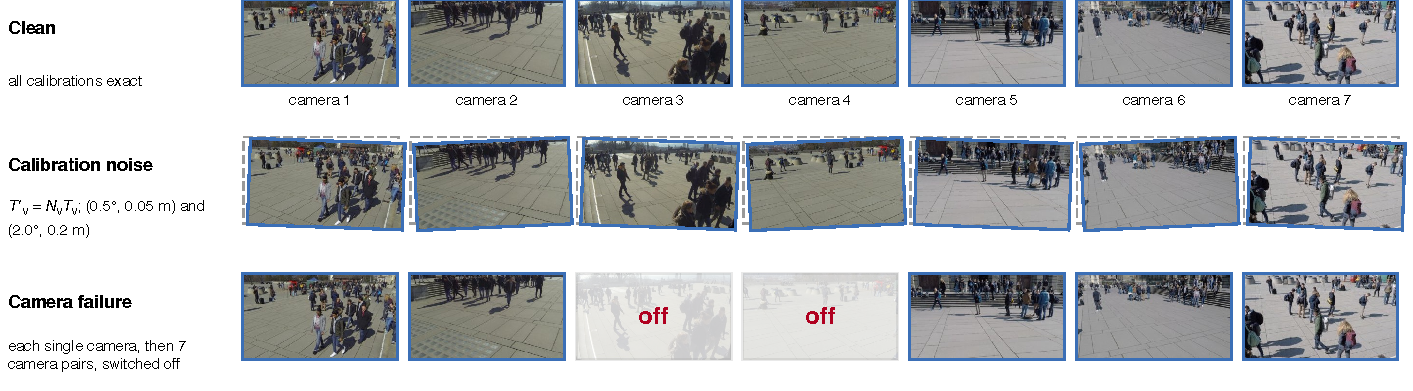
\includegraphics[width=0.9\textwidth]{figures/fig3_robustness.pdf}
  \caption{\textbf{Evaluation conditions.} All models are evaluated on the same test frames with exact calibration
  (top), with Gaussian noise on the extrinsics of every camera (middle; three fixed draws per noise level, shared by
  all models), and with one or two cameras switched off (bottom).}
  \label{fig:robust}
\end{figure*}

Because view mixing trains the network on partially misregistered evidence, we evaluate every trained model under
two perturbations of the test conditions (Fig.~\ref{fig:robust}); no model is retrained.

\paragraph{Calibration noise.} The extrinsics of each camera are perturbed in its own frame, $T'_v = N_v T_v$, where
$N_v$ combines a rotation whose axis-angle components are drawn from $\mathcal{N}(0, \sigma_r^2)$ with a translation
whose components are drawn from $\mathcal{N}(0, \sigma_t^2)$. We use
$(\sigma_r, \sigma_t) = (0.5^\circ, 0.05\,\mathrm{m})$ and $(2.0^\circ, 0.2\,\mathrm{m})$, the two noise levels
of~\cite[Tab.~5]{toida2025atlasfusion}. Three draws per level are fixed and shared by all models, so that models are
compared on identical perturbations.

\paragraph{Camera failure.} The lifted features of a switched-off camera are set to zero. We switch off each of the
seven cameras in turn, and then seven pairs of cameras.

For each condition we report MODA, MOTA and IDF1, averaged over the draws or camera subsets, and the seed-paired
difference between SA-VM and the baseline with the test of the previous subsection.

%-----------------------------------------------------------------------------------------------------------------
{\small
\begin{thebibliography}{99}

\bibitem{bernardin2008clear}
K.~Bernardin and R.~Stiefelhagen.
\newblock Evaluating multiple object tracking performance: The {CLEAR MOT} metrics.
\newblock {\em EURASIP Journal on Image and Video Processing}, 2008.

\bibitem{chavdarova2017wildtrack}
T.~Chavdarova, P.~Baqu\'e, S.~Bouquet, A.~Maksai, C.~Jose, L.~Lettry, P.~Fua, L.~Van~Gool, and F.~Fleuret.
\newblock The {WILDTRACK} multi-camera person dataset.
\newblock arXiv:1707.09299, 2017.

\bibitem{engilberge2023mvaug}
M.~Engilberge, H.~Shi, Z.~Wang, and P.~Fua.
\newblock Two-level data augmentation for calibrated multi-view detection.
\newblock In {\em WACV}, 2023.

\bibitem{harley2023simplebev}
A.~W. Harley, Z.~Fang, J.~Li, R.~Ambrus, and K.~Fragkiadaki.
\newblock Simple-{BEV}: What really matters for multi-sensor {BEV} perception?
\newblock In {\em ICRA}, 2023.

\bibitem{he2016resnet}
K.~He, X.~Zhang, S.~Ren, and J.~Sun.
\newblock Deep residual learning for image recognition.
\newblock arXiv:1512.03385, 2015.

\bibitem{hou2020mvdet}
Y.~Hou, L.~Zheng, and S.~Gould.
\newblock Multiview detection with feature perspective transformation.
\newblock In {\em ECCV}, 2020.

\bibitem{lin2017focal}
T.-Y. Lin, P.~Goyal, R.~Girshick, K.~He, and P.~Doll\'ar.
\newblock Focal loss for dense object detection.
\newblock arXiv:1708.02002, 2017.

\bibitem{ristani2016performance}
E.~Ristani, F.~Solera, R.~S. Zou, R.~Cucchiara, and C.~Tomasi.
\newblock Performance measures and a data set for multi-target, multi-camera tracking.
\newblock arXiv:1609.01775, 2016.

\bibitem{teepe2024lifting}
T.~Teepe, P.~Wolters, J.~Gilg, F.~Herzog, and G.~Rigoll.
\newblock Lifting multi-view detection and tracking to the bird's eye view.
\newblock In {\em CVPR Workshops}, 2024.

\bibitem{toida2025atlasfusion}
K.~Toida, T.~Sakai, T.~Nakamura, H.~Shimizu, and K.~Hotta.
\newblock {ATLASFusion}: Aggregation tracking with location-aware sparse fusion for robust spatio-temporal
multi-view pedestrian tracking.
\newblock arXiv:2509.08421, 2025.

\end{thebibliography}
}

\end{document}
